% Copyright 2018-2019 Melvin Eloy Irizarry-Gelpí
\setcounter{chapter}{6}
\chapter{Curved Mirrors}
%%%%%%%%%%%%%%%%%%%%%%%%%%%%%%%%%%%%%%%%%%%%%%%%%%%%%%%%%%%%%%%%%%%%%%%%%%%%%%%%
In this experiment you will learn about the properties of images produced by curved mirrors.
%%%%%%%%%%%%%%%%%%%%%%%%%%%%%%%%%%%%%%%%%%%%%%%%%%%%%%%%%%%%%%%%%%%%%%%%%%%%%%%%
\section{Preliminary}
%%%%%%%%%%%%%%%%%%%%%%%%%%%%%%%%%%%%%%%%%%%%%%%%%%%%%%%%%%%%%%%%%%%%%%%%%%%%%%%%
A mirror reflects light. Mirrors can be flat or curved. Flat mirrors are commonly found in bathrooms. Curved mirrors can either be concave or convex. As you will see, a concave mirror can produce a real image, in the sense that the image can be projected on a screen.

Light is emitted from an \textbf{object}. This light travels through space and then bounces of a mirror, potentially producing an \textbf{image} somewhere in space. There is a relationship between the distance between the object and the mirror, $d_{O}$, and the distance between the image and the mirror, $d_{I}$. This relationship involves a property of the mirror called the focal length $f$:
\begin{equation}
    \frac{1}{d_{O}} + \frac{1}{d_{I}} = \frac{1}{f}
\end{equation}
This is a curious relation because it involves the inverse quantities, and not the direct quantities themselves. Another way of writing this relation is as
\begin{equation}
    \frac{1}{d_{I}} = -\frac{1}{d_{O}} + \frac{1}{f}
\end{equation}
If you measure $d_{O}$ and $d_{I}$, then the chart with $1/d_{I}$ in the vertical axis and $1/d_{O}$ in the horizontal axis should have a linear shape. The slope of the line should be close to $-1$, and the value of the intercept should be close to the inverse of the focal length of the mirror used.

In practice it is easier to measure position than to measure distance. You have three things: the object, the image, and the mirror. Thus you have three positions along the track: the position $x_{O}$ of the object, the position $x_{I}$ of the image, and the position $x_{M}$ of the mirror. The distance between the object and the mirror is simply
\begin{equation}
    d_{O} = \left\vert x_{O} - x_{M} \right\vert
\end{equation}
Similarly, the distance between the image and the mirror is given by
\begin{equation}
    d_{I} = \left\vert x_{I} - x_{M} \right\vert
\end{equation}
%%%%%%%%%%%%%%%%%%%%%%%%%%%%%%%%%%%%%%%%%%%%%%%%%%%%%%%%%%%%%%%%%%%%%%%%%%%%%%%%
\subsection{Magnification}
%%%%%%%%%%%%%%%%%%%%%%%%%%%%%%%%%%%%%%%%%%%%%%%%%%%%%%%%%%%%%%%%%%%%%%%%%%%%%%%%
Curved mirrors produce images that look very different from the object that is emitting the light. Some differences can involve a change in \textbf{orientation}. For example, left and right can be switched, as is common with plane mirrors. Other differences can be a change in \textbf{size}. That is, the size of an image can be smaller or larger than the object. There is a quantity called magnification that is used to describe how the size of an image compares to the size of the object. Let $h_{I}$ be the height of the image, and $h_{O}$ be the height of the object. The magnification $m$ of the mirror is given by the ratio
\begin{equation}
    m = \frac{h_{I}}{h_{O}}
\end{equation}
Note that magnification has no units because it is the ratio of two lengths. There is another definition of the magnification that involves the distances from the mirror to the object and the image:
\begin{equation}
    m = \frac{d_{I}}{d_{O}}
\end{equation}
This particular definition is missing a minus sign that is traditionally used to denote a change in orientation. For practical purposes, you can ignore that minus sign.
%%%%%%%%%%%%%%%%%%%%%%%%%%%%%%%%%%%%%%%%%%%%%%%%%%%%%%%%%%%%%%%%%%%%%%%%%%%%%%%%
\section{Experiment}
%%%%%%%%%%%%%%%%%%%%%%%%%%%%%%%%%%%%%%%%%%%%%%%%%%%%%%%%%%%%%%%%%%%%%%%%%%%%%%%%
The experiment with the concave mirror consisted of recording the position of the mirror, the object, and the screen where the sharp image is projected. You also used a ruler to record the height of the object and the image.
%%%%%%%%%%%%%%%%%%%%%%%%%%%%%%%%%%%%%%%%%%%%%%%%%%%%%%%%%%%%%%%%%%%%%%%%%%%%%%%%
\section{Analysis}
%%%%%%%%%%%%%%%%%%%%%%%%%%%%%%%%%%%%%%%%%%%%%%%%%%%%%%%%%%%%%%%%%%%%%%%%%%%%%%%%
With the position of the object, mirror, and image you can calculate the distances $d_{O}$ and $d_{I}$. Then you can make a chart of $1 / d_{I}$ versus $1 / d_{O}$. The expected relation is
\begin{equation}
    \frac{1}{d_{I}} = -\frac{1}{d_{O}} + \frac{1}{f}
\end{equation}
The slope of the best fit line should be:
\begin{equation}
    \text{slope} = -1
\end{equation}
From the intercept you can find an experimental estimate of the focal length of the mirror:
\begin{equation}
    \text{focal length} = \frac{1}{\text{intercept}}
\end{equation}
The expected value for the focal length of the concave mirror used is 20 cm.

With the distances $d_{O}$ and $d_{I}$ you can calculate the magnification:
\begin{equation}
    m = \frac{d_{I}}{d_{O}}
\end{equation}
You can also calculate the magnification using the measured heights $h_{I}$ and $h_{O}$:
\begin{equation}
    m = \frac{h_{I}}{h_{O}}
\end{equation}
both of these methods should be consistent.
%%%%%%%%%%%%%%%%%%%%%%%%%%%%%%%%%%%%%%%%%%%%%%%%%%%%%%%%%%%%%%%%%%%%%%%%%%%%%%%%
\section{My Data}
%%%%%%%%%%%%%%%%%%%%%%%%%%%%%%%%%%%%%%%%%%%%%%%%%%%%%%%%%%%%%%%%%%%%%%%%%%%%%%%%
My data consist of ten distinct configurations. As can be seen from Figure \ref{figure.07.chart}, the expected behavior is observed between the inverse distances to the mirror. Further more, the slope and intercept agree with the expected values.

You can also see from Table \ref{table.07.magnification} that the two ways of computing the magnification of the mirror give similar results.
%%%%%%%%%%%%%%%%%%%%%%%%%%%%%%%%%%%%%%%%%%%%%%%%%%%%%%%%%%%%%%%%%%%%%%%%%%%%%%%%
\section{Your Data}
%%%%%%%%%%%%%%%%%%%%%%%%%%%%%%%%%%%%%%%%%%%%%%%%%%%%%%%%%%%%%%%%%%%%%%%%%%%%%%%%
You should have positions and heights for eight distinct configurations.
%%%%%%%%%%%%%%%%%%%%%%%%%%%%%%%%%%%%%%%%%%%%%%%%%%%%%%%%%%%%%%%%%%%%%%%%%%%%%%%%
\newpage
\section{Your Lab Report}
%%%%%%%%%%%%%%%%%%%%%%%%%%%%%%%%%%%%%%%%%%%%%%%%%%%%%%%%%%%%%%%%%%%%%%%%%%%%%%%%
Your laboratory report should include the following:
\begin{itemize}
    \item A table like Table \ref{table.07.magnification} with the magnification computed in two different ways.
    \item A chart with $d_{I}$ in the vertical axis, and $d_{O}$ in the horizontal axis.
    \item A chart with $1/d_{I}$ in the vertical axis, and $1/d_{O}$ in the horizontal axis. Include the best linear fit, and display the equation. See Figure \ref{figure.07.chart}.
    \item A table like Table \ref{table.07.results} with your results and the percent differences.
    \item Answer the following question: which method of calculating the magnification do you think is more accurate?
\end{itemize}
%%%%%%%%%%%%%%%%%%%%%%%%%%%%%%%%%%%%%%%%%%%%%%%%%%%%%%%%%%%%%%%%%%%%%%%%%%%%%%%%
\newpage
\section{Tables}
%%%%%%%%%%%%%%%%%%%%%%%%%%%%%%%%%%%%%%%%%%%%%%%%%%%%%%%%%%%%%%%%%%%%%%%%%%%%%%%%
\begin{table}[ht]
    \centering
    \begin{tabular}{|r|r|r|}
        \hline
        $x_{O}$ (cm) & $x_{M}$ (cm) & $x_{I}$ (cm) \\
        \hline
        10 & 120 & 96.05 \\
        10 & 112 & 87.35 \\
        10 & 104 & 79.1 \\
        10 & 96 & 70.15 \\
        10 & 88 & 61.35 \\
        10 & 80 & 52.55 \\
        10 & 72 & 43.05 \\
        10 & 64 & 32.5 \\
        10 & 56 & 21.35 \\
        60 & 90 & 36.2 \\
        \hline
    \end{tabular}
    \caption{Raw Position Data}
    \label{table.07.position}
\end{table}
%%%%%%%%%%%%%%%%%%%%%%%%%%%%%%%%%%%%%%%%%%%%%%%%%%%%%%%%%%%%%%%%%%%%%%%%%%%%%%%%
\begin{table}[ht]
    \centering
    \begin{tabular}{|r|r|}
        \hline
        $h_{O}$ (cm) & $h_{I}$ (cm) \\
        \hline
        2 & 0.5 \\
        2 & 0.5 \\
        2 & 0.5 \\
        2 & 0.7 \\
        2 & 0.7 \\
        2 & 0.8 \\
        2 & 0.9 \\
        2 & 1.1 \\
        2 & 1.4 \\
        2 & 3.5 \\
        \hline
    \end{tabular}
    \caption{Raw Height Data}
    \label{table.07.height}
\end{table}
%%%%%%%%%%%%%%%%%%%%%%%%%%%%%%%%%%%%%%%%%%%%%%%%%%%%%%%%%%%%%%%%%%%%%%%%%%%%%%%%
\begin{table}[ht]
    \centering
    \begin{tabular}{|r|r|}
        \hline
        $d_{O}$ (cm) & $d_{I}$ (cm) \\
        \hline
        110 & 23.95 \\
        102 & 24.65 \\
        94 & 24.9 \\
        86 & 25.85 \\
        78 & 26.65 \\
        70 & 27.45 \\
        62 & 28.95 \\
        54 & 31.5 \\
        46 & 34.65 \\
        30 & 53.8 \\
        \hline
    \end{tabular}
    \caption{Distances to the mirror}
    \label{table.07.distance}
\end{table}
%%%%%%%%%%%%%%%%%%%%%%%%%%%%%%%%%%%%%%%%%%%%%%%%%%%%%%%%%%%%%%%%%%%%%%%%%%%%%%%%
\begin{table}[ht]
    \centering
    \begin{tabular}{|r|r|}
        \hline
        $h_{I} / h_{O}$ & $d_{I} / d_{O}$ \\
        \hline
        0.25 & 0.22 \\
        0.25 & 0.24 \\
        0.25 & 0.26 \\
        0.35 & 0.30 \\
        0.35 & 0.34 \\
        0.4 & 0.39 \\
        0.45 & 0.45 \\
        0.55 & 0.58 \\
        0.7 & 0.75 \\
        1.75 & 1.79 \\
        \hline
    \end{tabular}
    \caption{Magnification}
    \label{table.07.magnification}
\end{table}
%%%%%%%%%%%%%%%%%%%%%%%%%%%%%%%%%%%%%%%%%%%%%%%%%%%%%%%%%%%%%%%%%%%%%%%%%%%%%%%%
\begin{table}[ht]
    \centering
    \begin{tabular}{|l|r|r|r|}
        \hline
        Name & Expected Value & Observed Value & P.D. (\%) \\
        \hline
        Slope & $-1$ & $-0.95$ & $-4.68$ \\
        Focal Length & 20 cm & 20.02 cm & $0.11$ \\
        \hline
    \end{tabular}
    \caption{Results}
    \label{table.07.results}
\end{table}
%%%%%%%%%%%%%%%%%%%%%%%%%%%%%%%%%%%%%%%%%%%%%%%%%%%%%%%%%%%%%%%%%%%%%%%%%%%%%%%%
\newpage
\FloatBarrier
\section{Figures}
%%%%%%%%%%%%%%%%%%%%%%%%%%%%%%%%%%%%%%%%%%%%%%%%%%%%%%%%%%%%%%%%%%%%%%%%%%%%%%%%
\begin{figure}[ht]
    \centering
    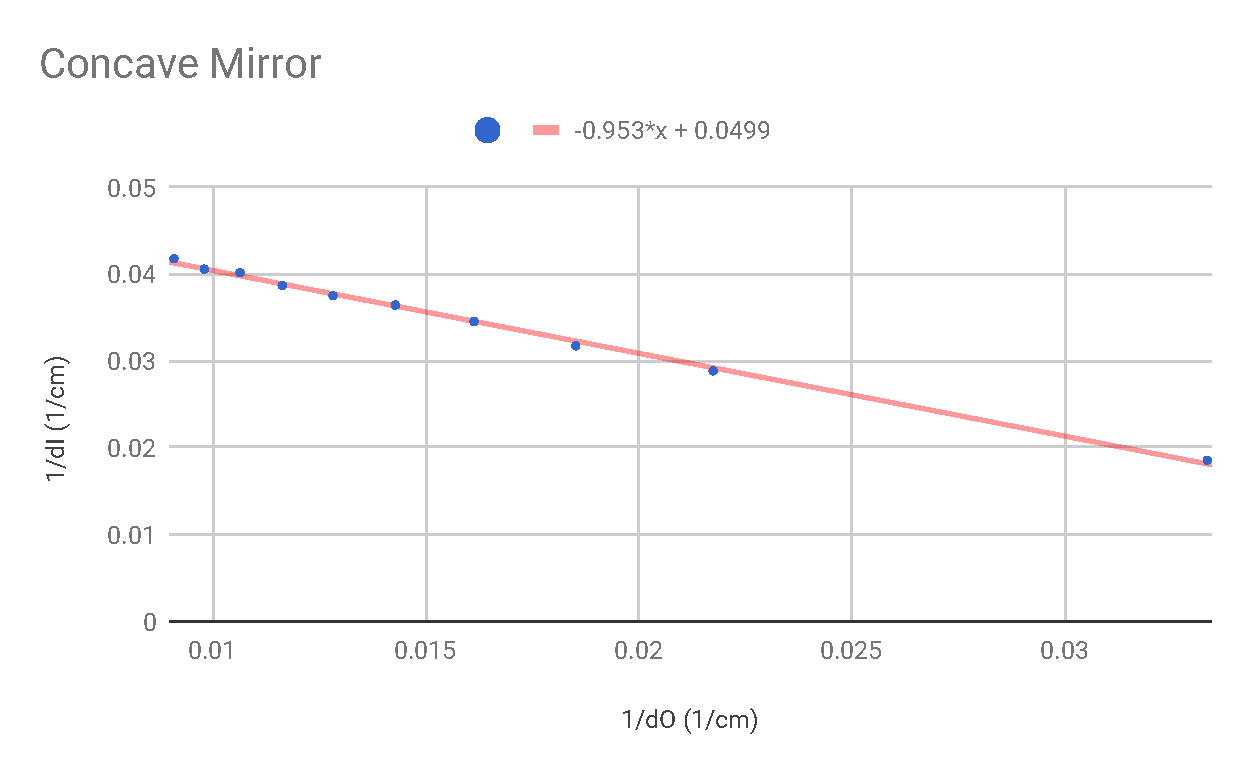
\includegraphics[scale=0.74]{image/07-mirrors/chart.pdf}
    \caption{Linear fit}
    \label{figure.07.chart}
\end{figure}
%%%%%%%%%%%%%%%%%%%%%%%%%%%%%%%%%%%%%%%%%%%%%%%%%%%%%%%%%%%%%%%%%%%%%%%%%%%%%%%%